\section{Suggestions for improvement}\label{jiveSuggestions}

Based on the mentioned shortcomings, the following improvements are suggested.
~\\

The ability to detect an inner type with a generic name, and display its parent type in the diagrams instead of its own.
This will make, among others, listener-heavy programs much more understandable as one can see what kind of listener each object is, instead of guessing, based on when it is invoked in the sequence-diagram.
Further helping the same situation, is to visually link listeners to the objects they are added to, in the contour-diagram, making it clearly visible which object is being listened to by the different listeners.
A crude visualization of these two changes, compared to the original, can be seen in \autoref{fig:contOving4Changes}.
~\\

Finding ways to highlight the different parts of e.g. an MVC-architecture, making it clearly visible which objects make out the models, views and controllers, may further help the understanding of a program.
But such highlighting must be balanced in order to not create a visual chaos of different colors.
Adding symbols instead of colors might be a better solution, both maintaining the current color-scheme, and adding new information.
The coloring, highlighting and naming of inner types should apply to both of the diagrams.
The biggest challenge with this kind of highlighting, is the process of detection.
While listeners can easily be detected by their implementation of a listener-interface, detecting a controller or a model is not trivial.
One can make assumptions based on class names, but they will be worthless if a program does not match those assumptions, and developers are not likely to change their programs to fit.
~\\
\begin{figure}[H]
	\centering
	\begin{subfigure}{\textwidth}
		\centering
		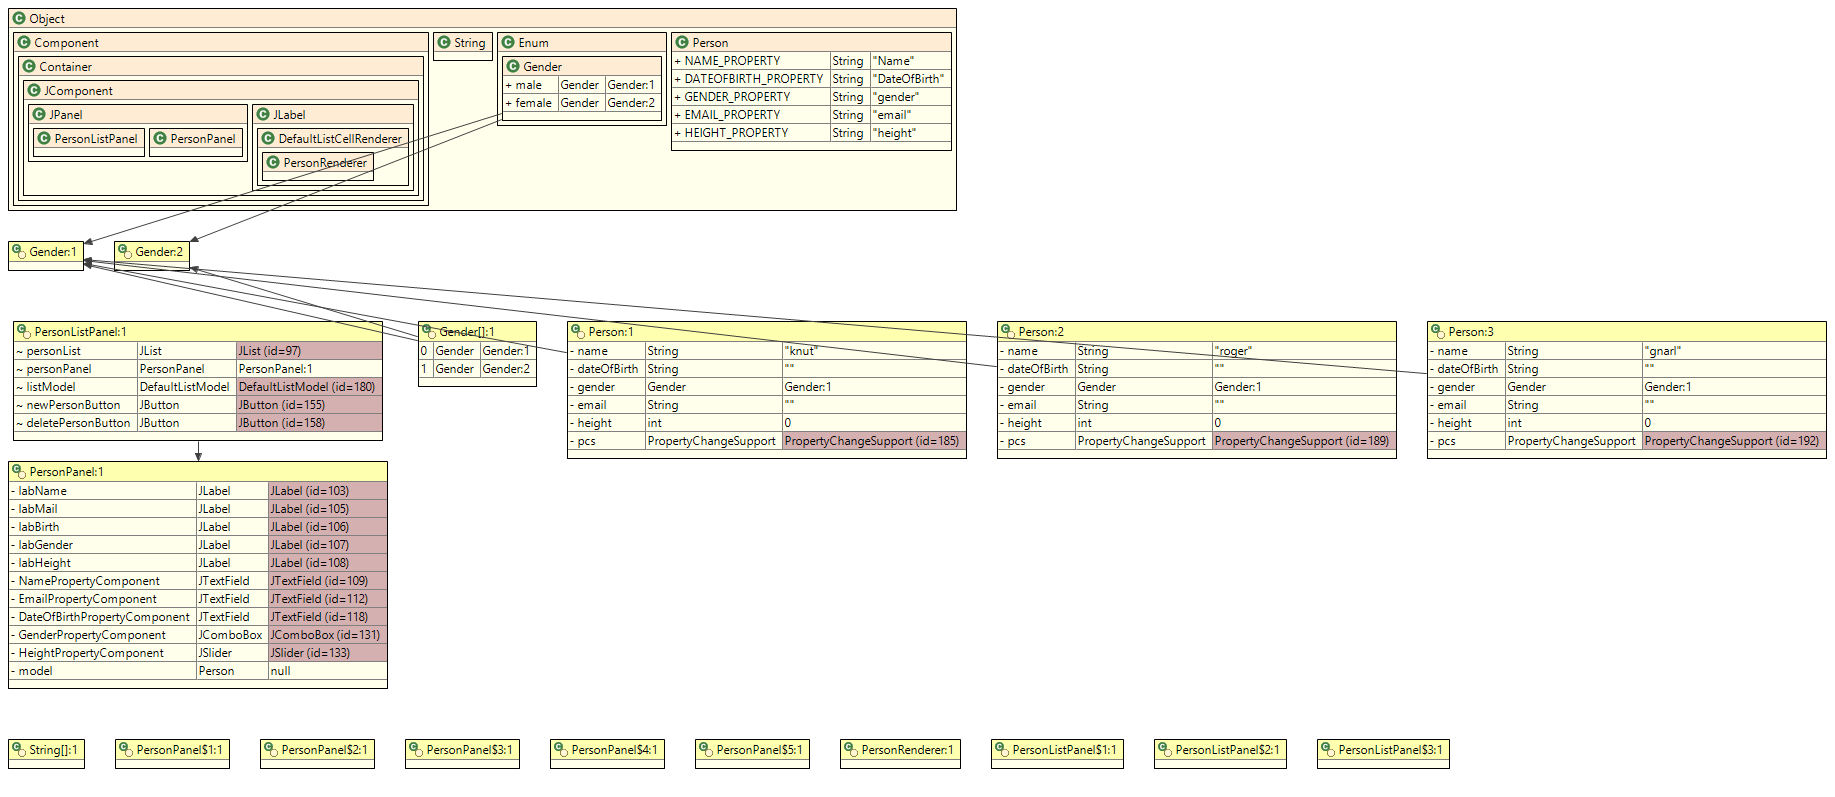
\includegraphics[width=\textwidth, trim= 0 0 0 0, clip]{MMI-Oving4-ObjectDiagInit}
		\caption{Original}
		\label{fig:contOving4ChangesA}
	\end{subfigure}
	\begin{subfigure}{\textwidth}
		\centering
		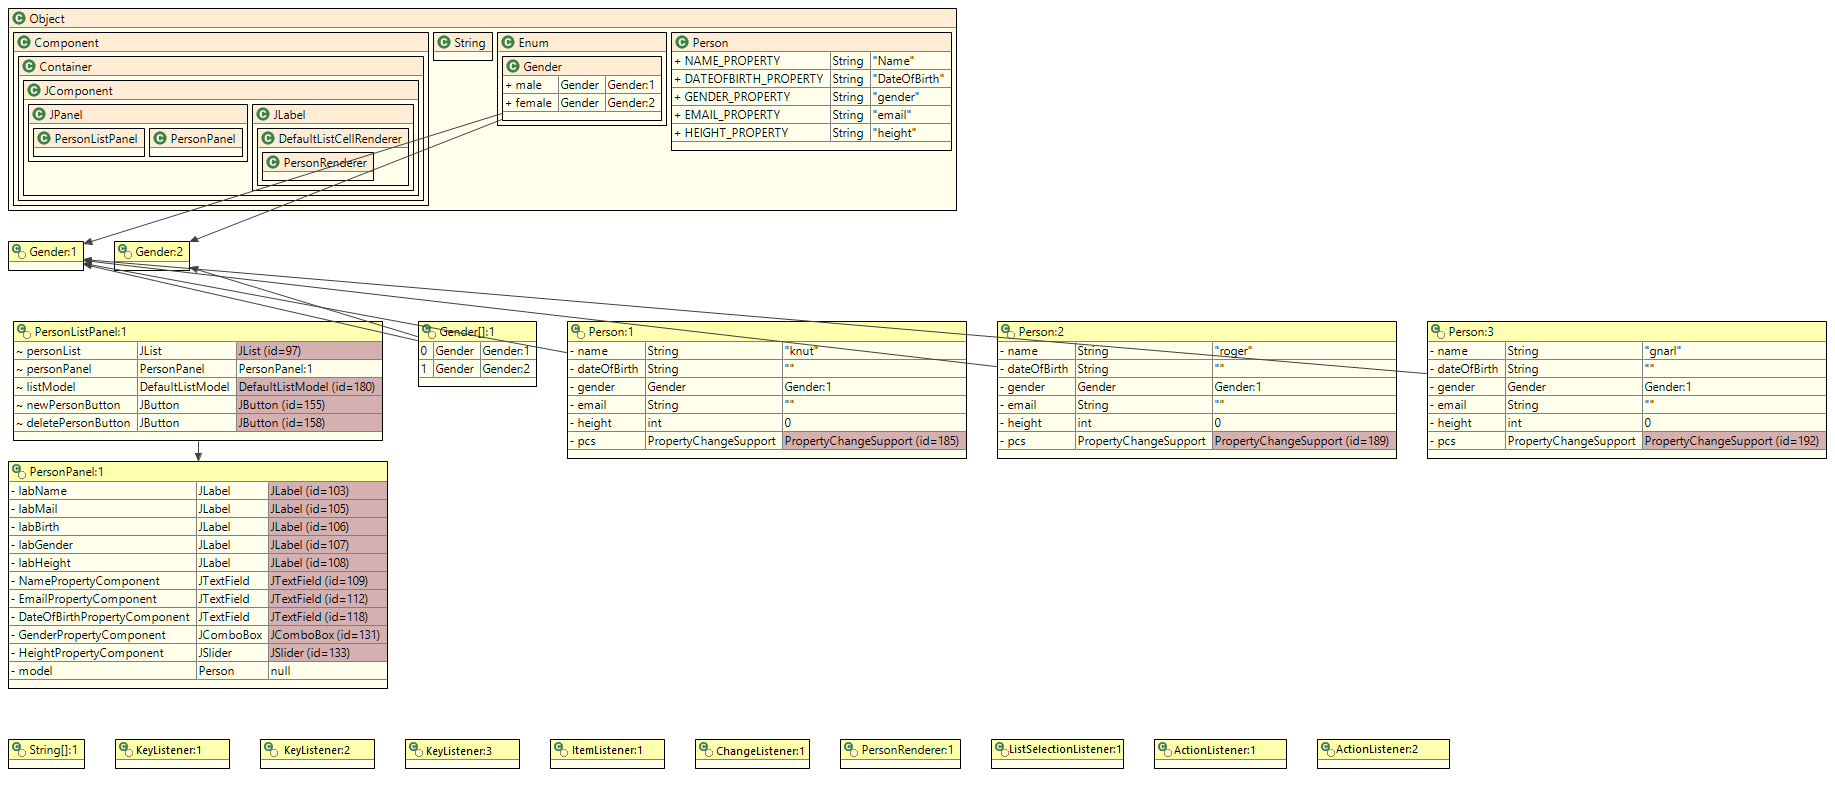
\includegraphics[width=\textwidth, trim= 0 0 0 0, clip]{MMI-Oving4-ObjectDiagInit-edit}
		\caption{Changed naming of inner types}
		\label{fig:contOving4ChangesB}
	\end{subfigure}
	\begin{subfigure}{\textwidth}
		\centering
		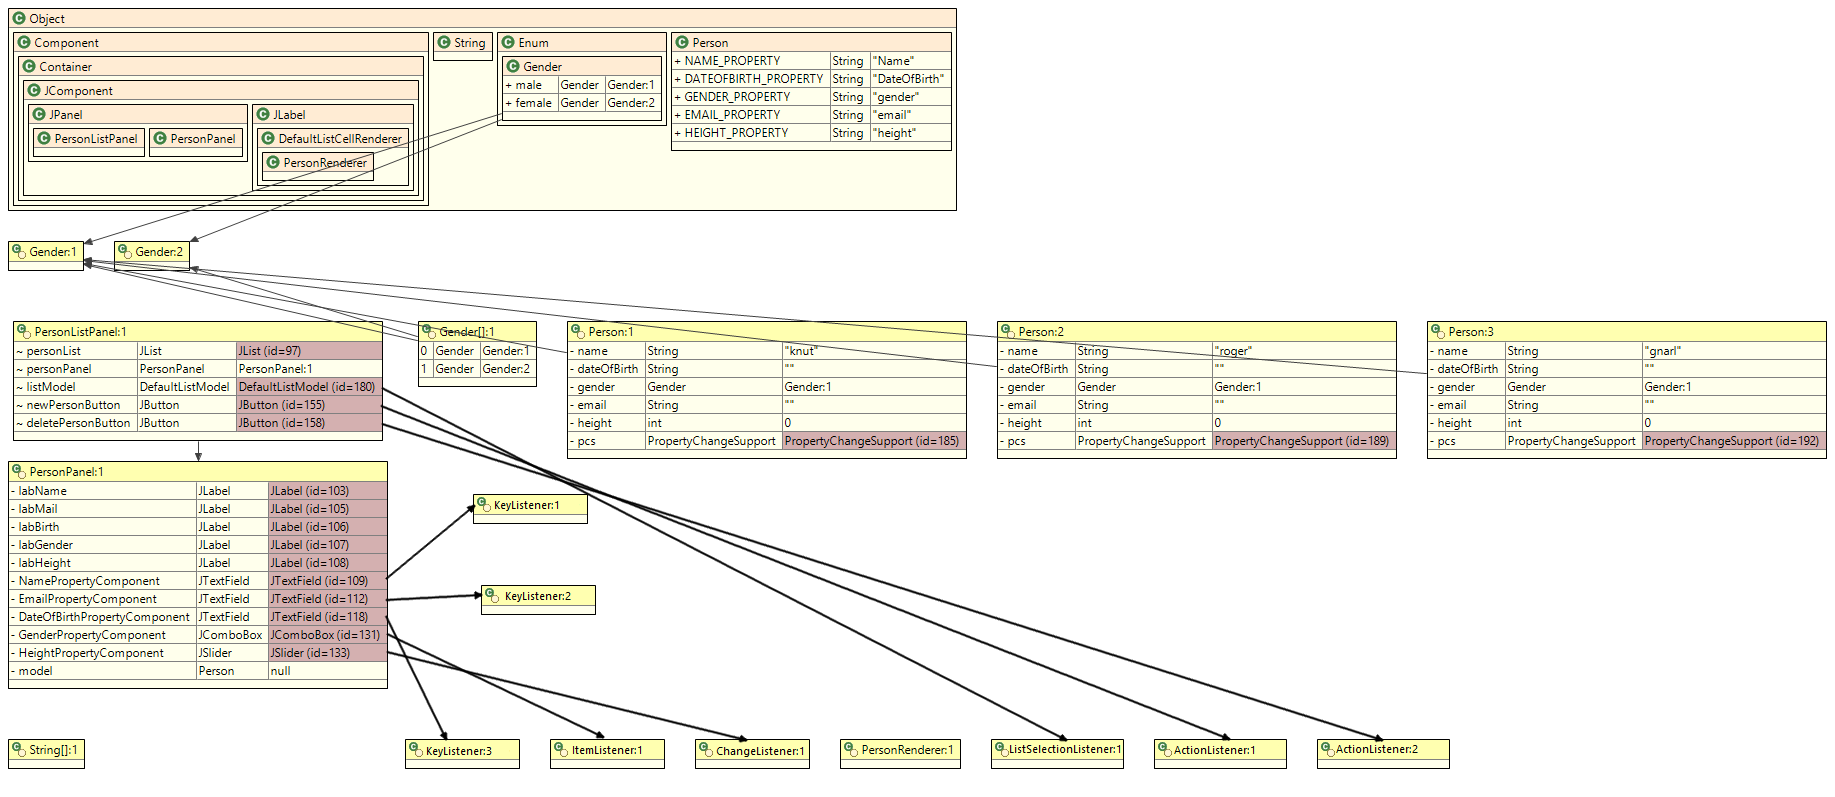
\includegraphics[width=\textwidth, trim= 0 0 0 0, clip]{MMI-Oving4-ObjectDiagInit-edit3}
		\caption{Listeners connected to the object listened to}
		\label{fig:contOving4ChangesC}
	\end{subfigure}
	\caption{Crude comparison of suggested changes to the contour diagram}
	\label{fig:contOving4Changes} 
\end{figure}
~\\

Exploring changes to the default exclusion-filter, in order to provide more useful information out of the box, is also an option.
This will provide a better experience for certain scenarios, but may be useless in other cases by providing too much unnecessary information.
A way to easily switch filters by defining presets might be preferable.
The filter might also be extended to support both exclusion and inclusion, allowing a more fine-grained selection of interesting classes.
As an example, one might be interested in ignoring the entire javax-package, but still allowing javax.swing in order to see more \gls{gui}-related objects.
It is also important to not allow too many packages through the filter, as the performance can suffer immensely from logging too many events.
~\\

Allowing more ways to interact with the diagrams, e.g. hiding elements or compressing sequences, should improve usability for larger programs and longer runs.
The way the sequence diagrams currently work, object instances are added as they appear, resulting in later method calls to draw lines crossing large parts of the diagram, as shown in \autoref{fig:seqOving4CrossLines}.
~\\

\begin{figure}[H]
	\centering
	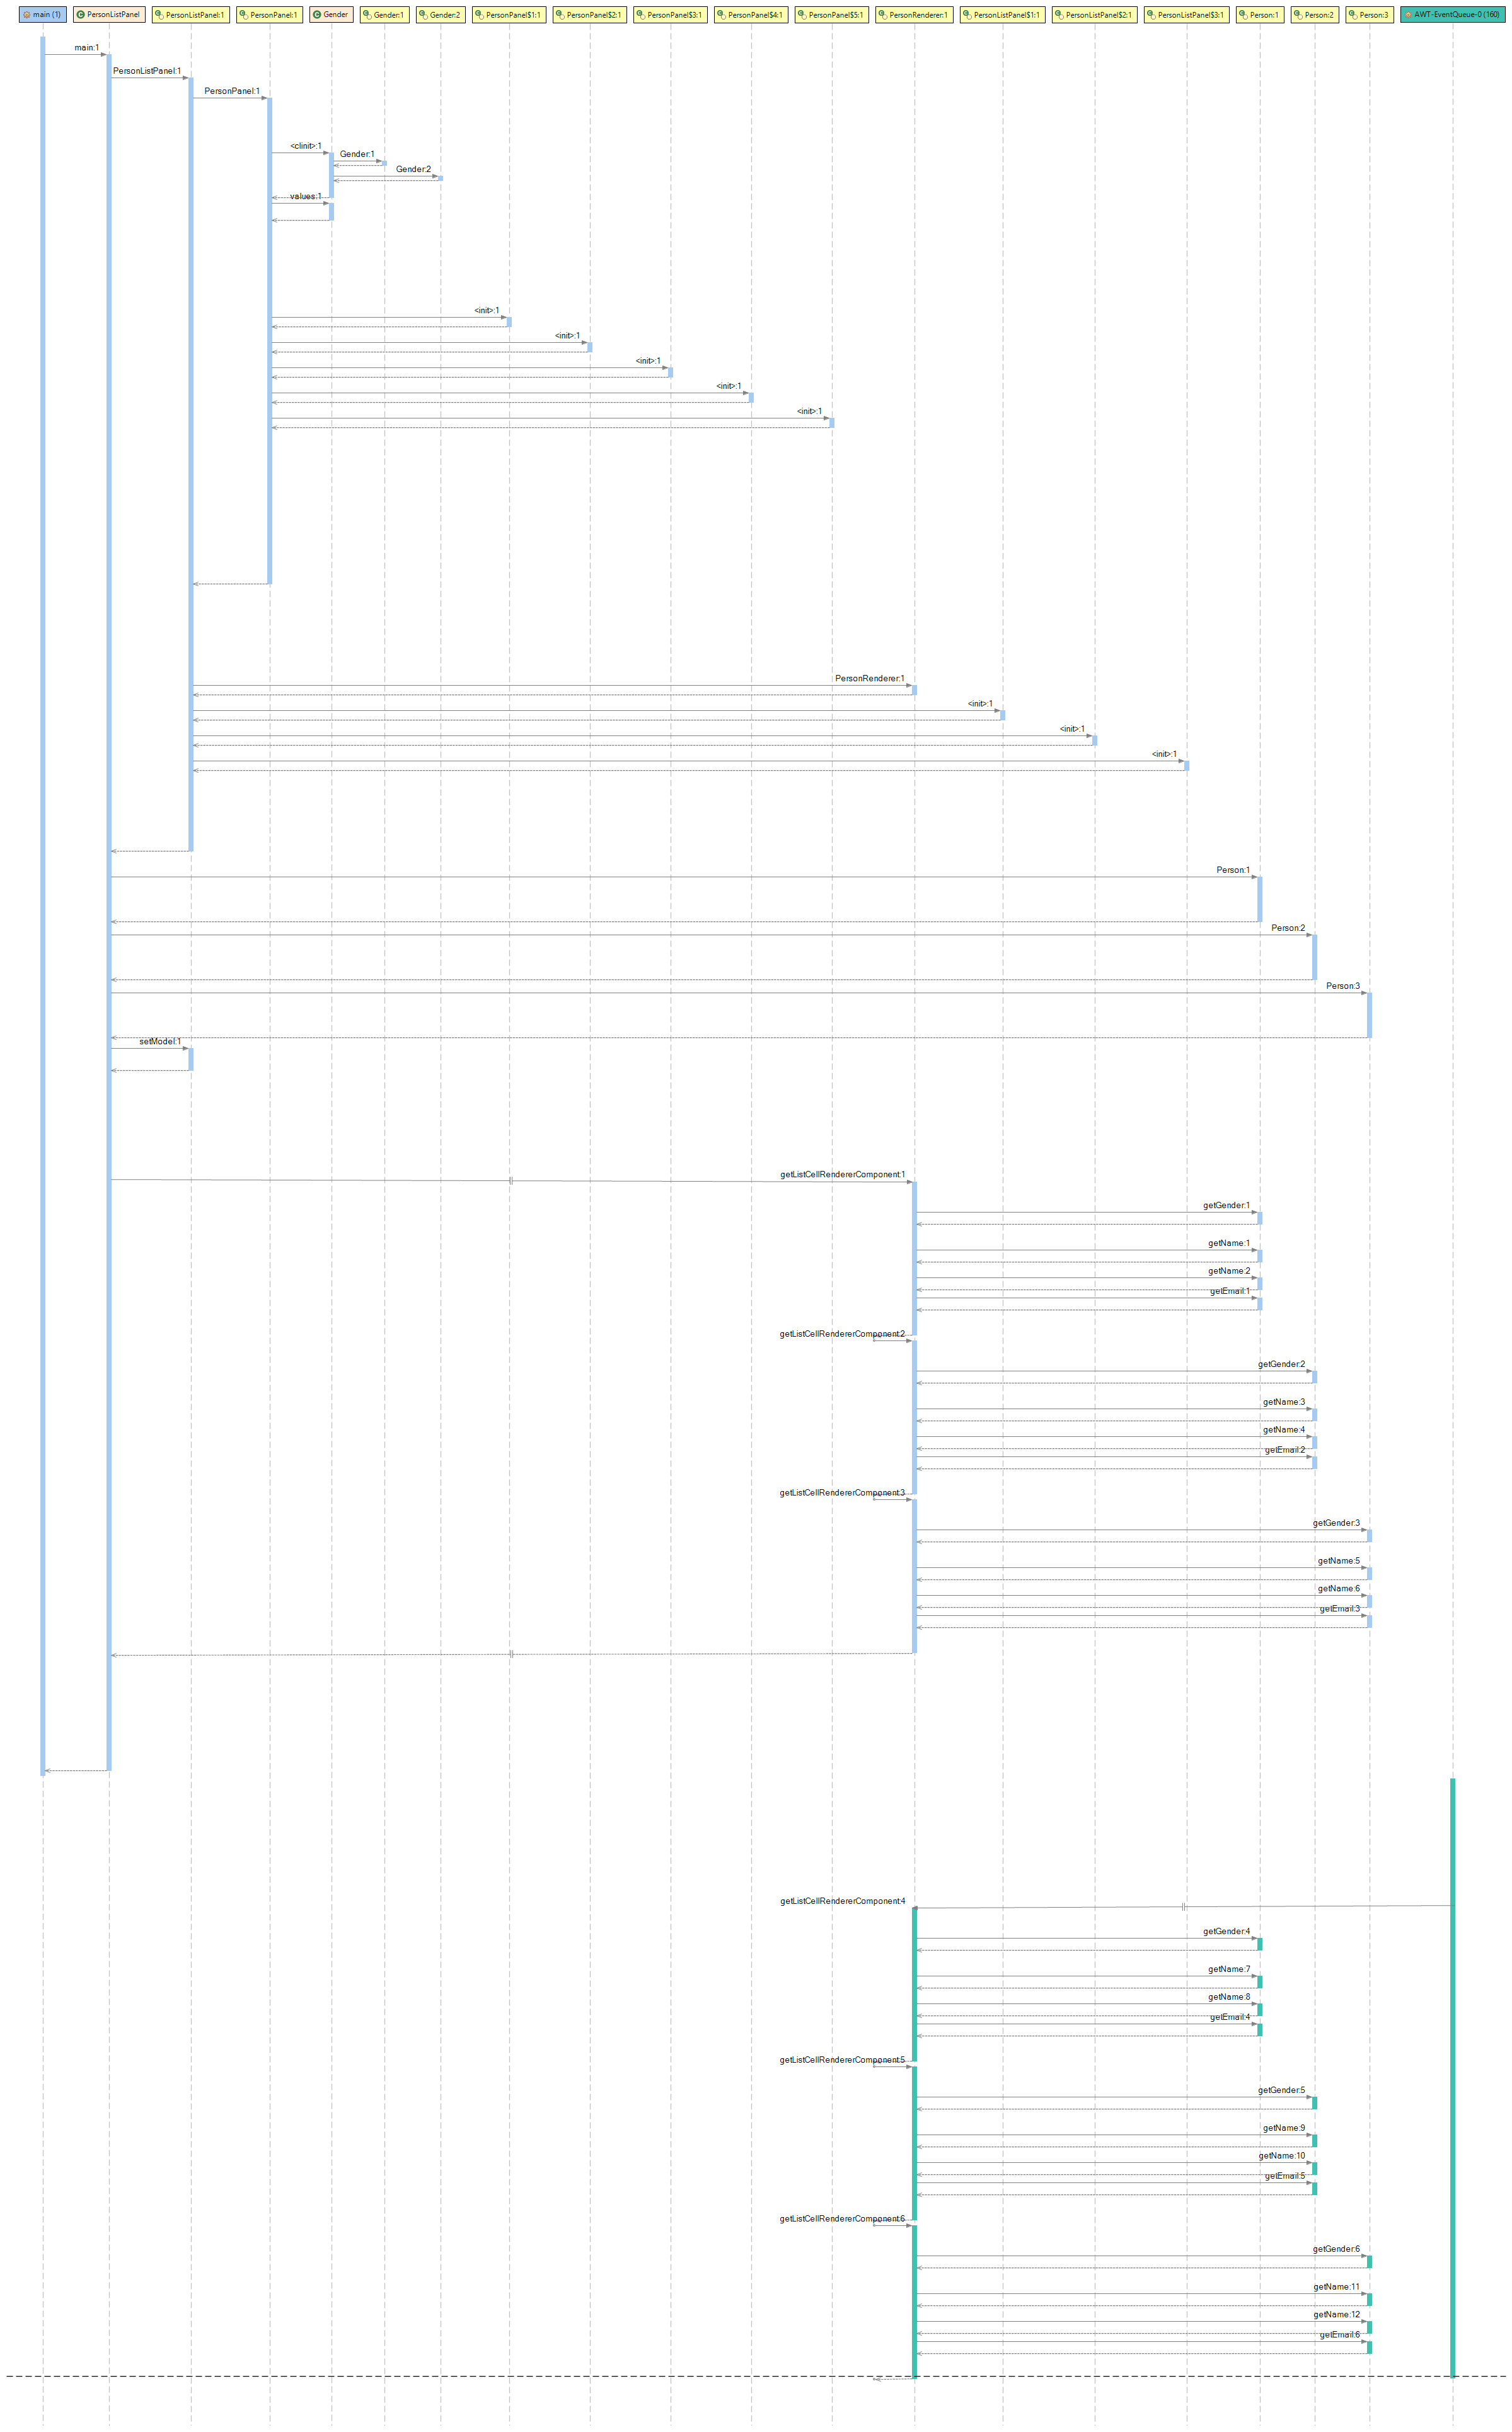
\includegraphics[width=\textwidth, trim= 45cm 7cm 0cm 103cm, clip]{MMI-Oving4-SequenceDiagInit}
	\caption{A section of a larger sequence diagram, showing method calls crossing several unrelated lifelines}
	\label{fig:seqOving4CrossLines}
\end{figure}
~\\

In the case of exploring events triggered by a listener, the ability to isolate the involved objects, and reorder the diagram could be very useful, providing a clean view of a smaller series of events.
Using the same figure as an example, the rightmost, and longest, bar would be moved to the far left, the three second-longest would be in the middle, while the shortest ones would be to the left.
In total, only the lifelines of those five objects would be visible, all the ones that are being crossed in \autoref{fig:seqOving4CrossLines} are unnecessary, and would be hidden as shown in \autoref{fig:seqOving4IsolatedMock}.
This function should be accessed by right clicking on the topmost event that is desired, and selecting a "view isolated" option.
Whether the isolated view should appear in a new eclipse view, or simply modify the existing view of the sequence diagram, is something that should be determined by user-testing.
~\\

\begin{figure}[H]
	\centering
	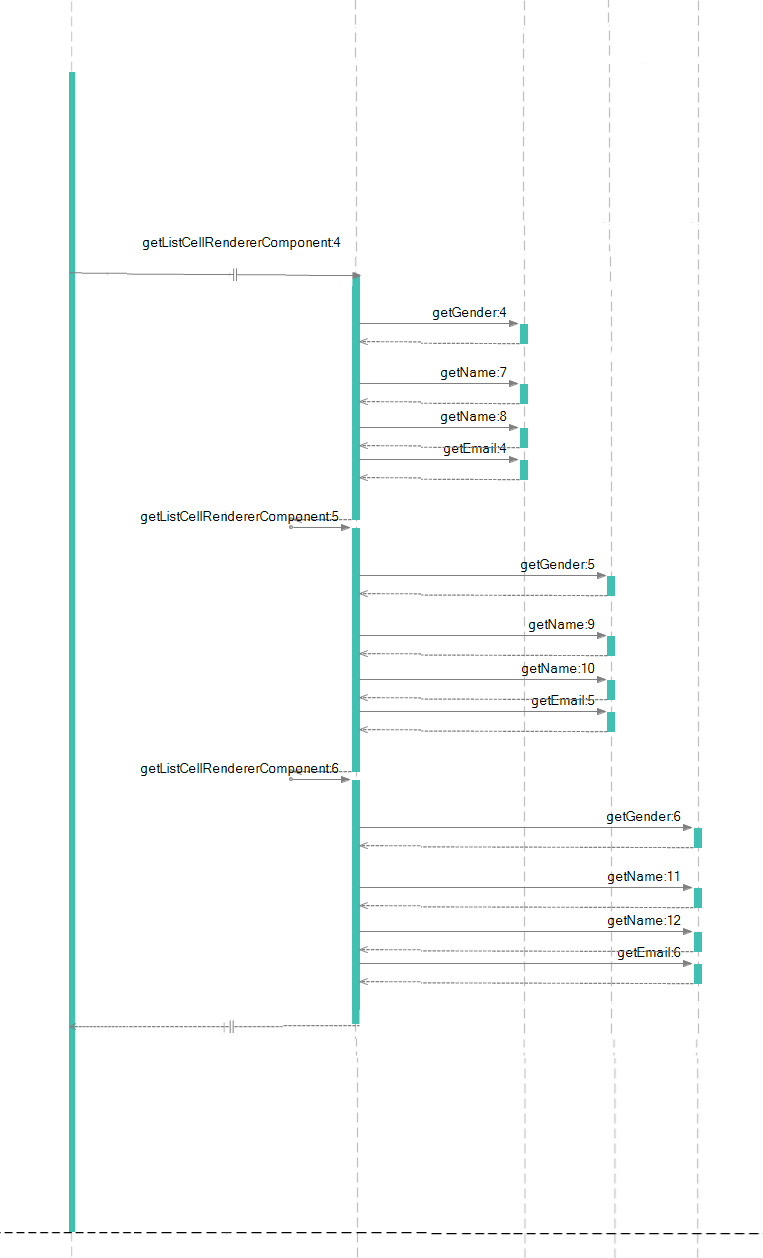
\includegraphics[height =.5\paperheight, trim= 0cm 5cm 0cm 5cm, clip]{MMI-Oving4-SequenceDiagInit-isolatedEventsMock}
	\caption{An example of how \autoref{fig:seqOving4CrossLines} might look in the isolated view}
	\label{fig:seqOving4IsolatedMock}
\end{figure}
~\\

Stepping through the recorded states is, as mentioned above, cumbersome.
While there are quick and easy ways to jump straight to any interesting state, it may also be interesting to view a playback of a part of, or the entire execution.
This would allow an easier way of observing changes happening in a program.
The playback would automatically step through the recorded states at a pace that the user should be able to adjust, updating the diagrams for each step.
Playback should be possible to initialize from any selected event that has been recorded, as starting from the beginning would often be a waste of time.
~\\

Searching can be improved by relaxing the requirements for for search-terms.
The requirement of full class names in searches caused some confusion, and made me wonder if the feature was working at all.
Relaxing this requirement to allowing partial class names, or substrings in general, would be an improvement to the usability of the tool.
~\\